\documentclass[a4paper, 11pt]{article}
\usepackage[
    top=0.75in,
    bottom=1in,
    left=0.75in,
    right=0.75in
]{geometry}
\usepackage{graphicx, tabularx, hyperref, amsmath, wrapfig}
\usepackage[siunitx]{circuitikz}
\usepackage{booktabs}
\usepackage{pgfplotstable, pgfplots}
%\renewcommand{\arraystretch}{1.2}
\linespread{1.2}
\selectfont
\usepackage{xepersian}
\settextfont[Scale=0.875]{Dibaj}
\setdigitfont[Scale=1]{Dibaj}


\begin{document}

\begin{center}
\textbf{{\huge گزارش‌کار آزمایش شمارهٔ
2: 
ﻗﻮاﻧﯿﻦ ﮐﯿﺮﺷﻬﻒ و ﭘﻞ وﺗﺴﺘﻮن
}}

\end{center}

\hrule
\noindent\begin{tabular}{rrl}
اعضای گروه: & ابوالفضل احمدی & 403172283\\
& نام و نام‌خانوادگی & 403001122
\end{tabular}\hfill
\begin{tabular}{rr}
تاریخ انجام آزمایش: & 17/08/1404 \\
دستیار آموزشی: & امیری‌نژاد \\
\end{tabular}\hfill
\begin{tabular}{rr}
گروه:  & 3 \\
زیرگروه: & \lr{A}  \\
\end{tabular}
\hrule

\section{اهداف و خلاصهٔ شرح آزمایش}

هدف کلی آزمایش، بررسی عملی قوانین کیرشهف و به‌کارگیری آن‌ها برای تحلیل مدارهای مقاومت در حضور دو منبع ولتاژ مستقل است. برای این منظور مراحل زیر انجام شد:

\begin{itemize}
    \item اندازه‌گیری مستقیم مقدار مقاومت‌های پنج‌گانه با مولتی‌متر به‌منظور داشتن مرجع عددی برای تحلیل مدار.
    \item بستن مدار شکل (1) با دو منبع \lr{$V_1$} و \lr{$V_2$}، اندازه‌گیری جریان شاخه‌ها و ولتاژ دو سر هر مقاومت، و آزمون کیفی و کمی قانون اول کیرشهف \lr{(KCL)} و قانون دوم کیرشهف \lr{(KVL)}.
    \item محاسبهٔ مقادیر تحلیلی جریان و افت پتانسیل هر شاخه با استفاده از قانون اهم و مقایسهٔ آن‌ها با داده‌های آزمایشگاهی برای برآورد درصد خطا و بررسی نقش خطاهای ابزاری و تلرانس مقاومت‌ها.
    \item تعیین مقاومت مجهول به دو روش: قانون اهم (اندازه‌گیری \lr{$V_{R_x}$} و \lr{$I_{R_x}$}) و تعادل پل وتستون، و سپس مقایسهٔ دو مقدار به‌همراه محاسبهٔ درصد اختلاف.
\end{itemize}

نتایج نشان داد جریان‌ها و ولتاژهای اندازه‌گیری‌شده با پیش‌بینی قوانین کیرشهف و قانون اهم هم‌خوانی خوبی دارند و اختلاف‌ها در حد خطاهای ابزاری و تلرانس قطعات باقی ماند. همچنین مقدار مقاومت مجهول به کمک پل وتستون با دقت بیشتری به‌دست آمد و تطابق مناسب با روش مستقیم داشت.

\section{تعیین اندازه مقاومت}
با استفاده از مولتی‌متر مقاومت‌ها را اندازه‌گیری کردیم و در جدول گزارش کردیم.
%\end{wraptable}{l}{4cm} % r = راست جدول، 4cm = پهنای جدول
%\vspace{-10pt} % برای تنظیم فاصله عمودی (اختیاری)
\begin{table}[h!]
\caption{}
\label{tab1}
\centering
\begin{tabular}{cc}
\hline
\multicolumn{2}{c}{مقاومت$\;[\mathrm{\Omega}]$} \\
\hline
$R_1$ & $388$ \\
$R_2$ & $219$ \\
$R_3$ & $47$ \\
$R_4$ & $46$ \\
$R_5$ & $99$ \\
\hline
\end{tabular}
\end{table}
%\end{wraptable}

\section{بررسی قوانین کیرشهف}

\begin{figure}[h]
\caption{}
\centering
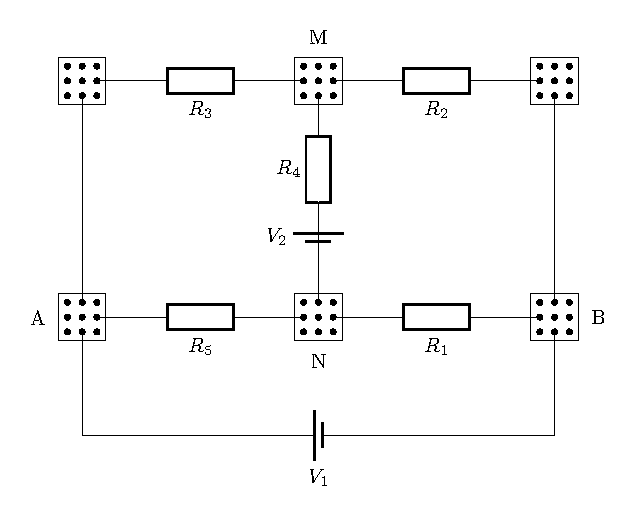
\includegraphics[width=14cm]{fig2.pdf}
\end{figure}

%\begin{wraptable}{l}{4cm} % r = راست جدول، 4cm = پهنای جدول
%\vspace{-30pt} % برای تنظیم فاصله عمودی (اختیاری)
\begin{table}[h!]
\caption{}
\label{tab2}
\centering
\begin{tabular}{cc}
\hline
\multicolumn{2}{c}{جریان هر شاخه$\;[\mathrm{mA}]$} \\
\hline
$I_{R_1}$ & $20.69$ \\
$I_{R_2}$ & $10.16$ \\
$I_{R_3}$ & $59.47$ \\
$I_{R_4}$ & $49.57$ \\
$I_{R_5}$ & $29.16$ \\
\hline
\end{tabular}
\end{table}
%\end{wraptable}

با استفاده از مقاومت‌های ارائه‌شده در جدول (1)، مداری مطابق با شکل (1) بسته شد. سپس با بهره‌گیری از ولت‌متر، ولتاژ منابع تغذیه به مقادیر \lr{$V_1 = 5\,\mathrm{V}$} و \lr{$V_2 = 8\,\mathrm{V}$} تنظیم گردید. در ادامه، به کمک آمپرمتر، جریان عبوری از هر یک از شاخه‌های مدار اندازه‌گیری شد و مقادیر به‌دست‌آمده در جدول (3) ثبت گردید. 


حال با استفاده از جریان‌های اندازه‌گیری‌شده، قانون اول کیرشهف مورد بررسی قرار می‌دهیم و صحت آن با مقایسهٔ مجموع جریان‌های ورودی و خروجی هر گره در مدار ارزیابی می‌کنیم.

\paragraph{بررسی قانون اول کیرشهف}

بر اساس قانون اول کیرشهف، در هر گره از مدار، مجموع جبری جریان‌های ورودی برابر با مجموع جبری جریان‌های خروجی است:
\begin{equation}
\sum I_{\text{in}} = \sum I_{\text{out}}.
\end{equation}

با توجه به شکل (2)، یک گرهٔ مشترک در مدار در نظر می‌گیریم	 که جریان عبوری از مقاومت \lr{$R_4$} به‌عنوان جریان خروجی به گره و جریان‌های عبوری از مقاومت‌های 
 \lr{$R_1$} و \lr{$R_5$} به‌عنوان جریان‌های ,ورودی از گره در نظر گرفته می‌شوند. با ملاحظه مقادیر جریان‌های اندازه‌گیری‌شده (جدول \ref{tab2}) 
مجموع جریان‌های ورودی از گره برابر است با:
\begin{align}
\sum I_{\text{in}} &= I_{R_1} + I_{R_5} \nonumber\\
&= 20.69 + 29.16 \nonumber\\
&= 49.16~\mathrm{mA}.
\end{align}

و جریان خروجی به گره برابر است با:
\begin{equation}
\sum I_{\text{out}} = I_{R_4} = 49.57~\mathrm{mA}.
\end{equation}

مشاهده می‌شود که مجموع جریان‌های ورودی و خروجی به‌طور تقریبی برابر هستند. اختلاف بین آن‌ها به صورت زیر محاسبه می‌شود:
\begin{equation}
\Delta I = \left| \sum I_{\text{out}} - \sum I_{\text{in}} \right|
= |4.16 - 49.57|
= 0.41~\mathrm{mA}.
\end{equation}

این اختلاف می‌تواند ناشی از عوامل زیر باشد:
\begin{itemize}
\item خطای اندازه‌گیری آمپرمتر (محدودیت دقت دستگاه)،
\item مقاومت داخلی آمپرمتر و سیم‌های رابط،
\item نوسان ولتاژ منابع تغذیه،
\item تلرانس مقاومت‌ها و تغییر مقدار آن‌ها در اثر گرم‌شدن،
\item یا در نظر نگرفتن دقیق جهت جریان‌ها در تحلیل گره.
\end{itemize}

با در نظر گرفتن این عوامل، می‌توان نتیجه گرفت که قانون اول کیرشهف به‌صورت کیفی در مدار برقرار است و اختلاف مشاهده‌شده در محدودهٔ خطاهای آزمایشگاهی قابل توجیه می‌باشد.

برای گره بعدی، گره‌ای را در نظر می‌گیریم که جریان عبوری از مقاومت $R_3$ به عنوان جریان خروجی به گره و جریان‌های عبوری از مقاومت‌های $R_2$ و $R_4$ به عنوان جریان‌های ورودی از گره در نظر گرفته می‌وشند. پس جریان‌های ورودی به گره برابر است با:

\begin{align}
\sum I_{\text{in}} &= I_{R_2} + I_{R_4} \nonumber\\
&= 10.16 + 49.57 \nonumber\\
&= 59.73~\mathrm{mA}.
\end{align}

و خروجی:

\begin{equation}
\sum I_{\text{out}} = I_{R_3} = 59.47~\mathrm{mA}.
\end{equation}

که اختلاف آن‌ها برابر است با:
\begin{equation}
\Delta I = \left| \sum I_{\text{out}} - \sum I_{\text{in}} \right|
= | 59.73 - 59.47 |
= 0.26 \mathrm{mA}
\end{equation}

در ادامهٔ آزمایش، افت پتانسیل دو سر هر یک از مقاومت‌های مدارِ شکل (2) با استفاده از ولت‌متر اندازه‌گیری شد و مقادیر حاصل در جدول (4) ثبت گردید. 

%\end{wraptable}{l}{4cm} % r = راست جدول، 4cm = پهنای جدول
%\vspace{-10pt} % برای تنظیم فاصله عمودی (اختیاری)
\begin{table}[h!]
\caption{}
\label{tab3}
\centering
\begin{tabular}{cc}
\hline
\multicolumn{2}{c}{افت پتانسیل دو سر مقاومت$\;[\mathrm{V}]$} \\
\hline
$V_{R_1}$ & $7.96$ \\
$V_{R_2}$ & $2.24$ \\
$V_{R_3}$ & $2.82$ \\
$V_{R_4}$ & $2.28$ \\
$V_{R_5}$ & $2.89$ \\
\hline
\end{tabular}
\end{table}
%\end{wraptable}

اکنون با تکیه بر ولتاژهای اندازه‌گیری‌شده، قانون دوم کیرشهف برای هر مسیر بسته (حلقه) مورد بررسی قرار می‌دهیم و با محاسبهٔ جبری مجموع افت ولتاژها و مقایسهٔ آن با ولتاژ منبع(ها)، میزان انطباق نتایج با این قانون ارزیابی می‌کنیم.

\paragraph{بررسی قانون دوم کیرشهف \lr{(KVL)}}

بر اساس قانون دوم کیرشهف، در هر مسیر بسته (حلقه) جمع جبری تغییرات پتانسیل برابر صفر است. به بیان دیگر، در یک حلقهٔ بسته، مجموع ولتاژهای منابع با مجموع افت ولتاژهای عناصر مصرف‌کننده (مقاومت‌ها) برابر می‌شود:
\begin{equation}
\sum \Delta V = 0 
\qquad \Longleftrightarrow \qquad
\sum V_{\text{منبع}} = \sum V_{\text{افت}}.
\end{equation}
در این آزمایش افت پتانسیل دو سر مقاومت‌ها مطابق جدول \ref{tab3} اندازه‌گیری شد و سپس \lr{KVL} برای حلقه‌های مدار شکل (2) بررسی گردید. قرارداد علامت‌گذاری به این صورت در نظر گرفته شد که عبور از منبع از قطب منفی به مثبت، افزایش پتانسیل \lr{$(+V)$} و عبور از مقاومت در جهت جریان، افت پتانسیل \lr{$(-V_R)$} محسوب شود.

\subparagraph{حلقهٔ شامل منبع \texorpdfstring{$V_2$}{V2}}
برای حلقه‌ای که شامل منبع \lr{$V_2=8\,\mathrm{V}$} و مقاومت‌های $R_1$ ، $R_2$ و $R_4$ است، رابطهٔ \lr{KVL} به صورت زیر نوشته می‌شود:
\begin{equation}
+V_2 - V_{R_4} - V_{R_2} - V_{R_1} = 0.
\end{equation}
با جایگذاری مقدار اندازه‌گیری‌شده:
\begin{align}
S_{(V_2)} &= V_2 - V_{R_4} - V_{R_2} - V_{R_1}\nonumber\\
&= V_2 - 2.28 + 2.24 -7.96 \nonumber\\
&= 8 - 8.00 = 0 \mathrm{V}
\end{align}


برای حلقه‌ای که شامل منبع \lr{$V_2=8\,\mathrm{V}$} و مقاومت‌های $R_3$ ، $R_4$ و $R_5$ است، رابطهٔ \lr{KVL} به صورت زیر نوشته می‌شود:
\begin{equation}
+V_2 - V_{R_4} - V_{R_3} - V_{R_5} = 0.
\end{equation}
با جایگذاری مقدار اندازه‌گیری‌شده:
\begin{align}
S_{(V_2)} &= V_2 - V_{R_4} - V_{R_3} - V_{R_5}\nonumber\\
&= V_2 - 2.28 - 2.82 - 2.89\nonumber\\
&= 8 - 7.99 = 0.01 \mathrm{V}
\end{align}
در نتیجه درصد عدم انطباق نسبت به ولتاژ منبع \lr{$V_2$} برابر است با:
\begin{equation}
\%\text{خطا}_{(V_2)}=
\left|\frac{S_{(V_2)}}{V_2}\right|\times 100
=
\left|\frac{0.01}{8.00}\right|\times 100
= 0.125\%.
\end{equation}


\subparagraph{حلقهٔ شامل منبع \texorpdfstring{$V_1$}{V1} (مسیر \texorpdfstring{$R_2$}{R2} و \texorpdfstring{$R_3$}{R3})}
برای حلقه‌ای که شامل منبع \lr{$V_1=5\,\mathrm{V}$} و مقاومت‌های \lr{$R_2$} و \lr{$R_3$} است:
\begin{equation}
+V_1 - V_{R_2} - V_{R_3} = 0.
\end{equation}
با جایگذاری مقادیر جدول \ref{tab3}:
\begin{align}
S_{(R_2R_3)} &= V_1 - (V_{R_2}+V_{R_3}) \nonumber\\
&= 5.00 - (2.24 + 2.82) \nonumber\\
&= 5.00 - 5.06 = -0.06~\mathrm{V}.
\end{align}
بنابراین درصد عدم انطباق نسبت به \lr{$V_1$} برابر است با:
\begin{equation}
\%\text{خطا}_{(R_2R_3)}=
\left|\frac{S_{(R_2R_3)}}{V_1}\right|\times 100
=
\left|\frac{-0.06}{5.00}\right|\times 100
= 1.2\%.
\end{equation}

\subparagraph{حلقهٔ شامل منبع \texorpdfstring{$V_1$}{V1} (مسیر \texorpdfstring{$R_4$}{R4} و \texorpdfstring{$R_5$}{R5})}
برای حلقه‌ای که شامل منبع \lr{$V_1=5\,\mathrm{V}$} و مقاومت‌های \lr{$R_4$} و \lr{$R_5$} است:
\begin{equation}
+V_1 - V_{R_1} - V_{R_5} = 0.
\end{equation}
با جایگذاری:
\begin{align}
S_{(R_1R_5)} &= V_1 - V_{R_1} - V_{R_5} \nonumber\\
&= 5.00 - 7.96 + 2.89 \nonumber\\
&= 5.00 - 5.07 = -0.07~\mathrm{V}.
\end{align}
و درصد عدم انطباق:
\begin{equation}
\%\text{خطا}_{(R_4R_5)}=
\left|\frac{S_{(R_1R_5)}}{V_1}\right|\times 100
=
\left|\frac{-0.07}{5.00}\right|\times 100
= 1.4\%.
\end{equation}

نتایج به‌دست‌آمده نشان می‌دهد که در حلقه‌های بررسی‌شده، مجموع افت ولتاژهای اندازه‌گیری‌شده با ولتاژ منبع(ها) اختلاف کوچکی (در حد چند صدم تا چند دهم ولت) دارد. این اختلاف‌ها می‌تواند ناشی از مقاومت داخلی منابع تغذیه، مقاومت داخلی ولت‌متر، افت ولتاژ روی سیم‌های رابط و اتصالات، تلرانس مقاومت‌ها و خطای قرائت باشد. بنابراین، قانون دوم کیرشهف در محدودهٔ دقت ابزارها و شرایط آزمایش، با داده‌های اندازه‌گیری‌شده سازگار ارزیابی می‌شود.

 حال با استفاده از مقادیر معلوم مقاومت‌ها و ولتاژ منابع تغذیه، جریان عبوری از هر شاخه و افت پتانسیل مربوط به هر مقاومت به روش تحلیلی (به‌کارگیری قوانین گره و حلقه و روابط اهم) محاسبه می‌کنیم و در نهایت، نتایج محاسبه‌شده با داده‌های آزمایش مقایسه و خطای هر کمیت (جریان و افت پتانسیل) گزارش می‌کنیم.

\paragraph{محاسبات تحلیلی جریان‌ها و افت پتانسیل‌ها برای تمامی شاخه‌ها و مقایسه با آزمایش}

حال برای تمامی شاخه‌هایی که در بخش قبل بررسی شدند (مقاومت‌های $R_1$ تا $R_5$)، جریان و افت پتانسیل به روش تحلیلی و با استفاده از قانون اهم محاسبه می‌کنیم و سپس با مقادیر اندازه‌گیری‌شده مقایسه می‌کنیم. از آنجا که برای هر مقاومت مقدار $R_i$ (جدول \ref{tab1}) و همچنین ولتاژ اندازه‌گیری‌شدهٔ دو سر آن $V_{R_i}$ (جدول \ref{tab3}) و جریان شاخه $I_{R_i}$ (جدول \ref{tab2}) در دسترس است، دو بررسی مستقل انجام می‌شوند:

\begin{itemize}
\item \textbf{محاسبهٔ جریان تحلیلی از روی ولتاژ اندازه‌گیری‌شده:}
\begin{equation}
I_{R_i}^{(\mathrm{theo})} = \frac{V_{R_i}^{(\mathrm{exp})}}{R_i},
\label{eq:Itheo}
\end{equation}

\item \textbf{محاسبهٔ ولتاژ تحلیلی از روی جریان اندازه‌گیری‌شده:}
\begin{equation}
V_{R_i}^{(\mathrm{theo})} = I_{R_i}^{(\mathrm{exp})}\,R_i.
\label{eq:Vtheo}
\end{equation}
\end{itemize}

در نهایت، درصد خطا برای جریان و ولتاژ هر شاخه به‌ترتیب از روابط زیر محاسبه خواهند شد:
\begin{align}
\%\text{خطا}_{I,i} &=
\left|\frac{I_{R_i}^{(\mathrm{exp})}-I_{R_i}^{(\mathrm{theo})}}{I_{R_i}^{(\mathrm{theo})}}\right|\times 100,
\label{eq:errI}
\\
\%\text{خطا}_{V,i} &=
\left|\frac{V_{R_i}^{(\mathrm{exp})}-V_{R_i}^{(\mathrm{theo})}}{V_{R_i}^{(\mathrm{theo})}}\right|\times 100.
\label{eq:errV}
\end{align}

\paragraph{محاسبات عددی (برای تمام شاخه‌ها)}
ابتدا جریان تحلیلی هر شاخه با استفاده از رابطهٔ \eqref{eq:Itheo} محاسبه می‌شوند. به عنوان نمونه برای مقاومت $R_1$:
\[
I_{R_1}^{(\mathrm{theo})}=\frac{V_{R_1}^{(\mathrm{exp})}}{R_1}
=\frac{7.96}{388}
=0.020515~\mathrm{A}
=20.515~\mathrm{mA}.
\]
به همین ترتیب، سایر شاخه‌ها نیز محاسبه می‌شوند. همچنین ولتاژ تحلیلی هر شاخه با استفاده از رابطهٔ \eqref{eq:Vtheo} به‌دست می‌آید.

\begin{table}[h!]
\centering
\caption{مقایسهٔ مقادیر تحلیلی و تجربی برای جریان و افت پتانسیل در شاخه‌های مختلف}
\label{tab:compare}
\begin{tabular}{cccccccc}
\hline
مقاومت & $R~[\Omega]$ &
$V^{(\mathrm{exp})}~[\mathrm{V}]$ &
$I^{(\mathrm{exp})}~[\mathrm{mA}]$ &
$I^{(\mathrm{theo})}=\frac{V}{R}~[\mathrm{mA}]$ &
$\%\text{خطا}_I$ &
$V^{(\mathrm{theo})}=IR~[\mathrm{V}]$ &
$\%\text{خطا}_V$ \\
\hline
$R_1$ & $388$ & $7.96$ & $20.69$ & $20.515$ & $0.851\%$ & $8.028$ & $0.844\%$ \\
$R_2$ & $219$ & $2.24$ & $10.16$ & $10.228$ & $0.668\%$ & $2.225$ & $0.672\%$ \\
$R_3$ & $47$  & $2.82$ & $59.47$ & $60.000$ & $0.883\%$ & $2.795$ & $0.891\%$ \\
$R_4$ & $46$  & $2.28$ & $49.57$ & $49.565$ & $0.010\%$ & $2.280$ & $0.010\%$ \\
$R_5$ & $99$  & $2.89$ & $29.16$ & $29.192$ & $0.109\%$ & $2.887$ & $0.109\%$ \\
\hline
\end{tabular}
\end{table}

مطابق جدول \ref{tab:compare}، اختلاف بین مقادیر تحلیلی و تجربی برای جریان‌ها و افت پتانسیل‌ها در تمامی شاخه‌ها کوچک بوده و (در این داده‌ها) حداکثر در حدود $1\%$ است. این نتیجه نشان می‌دهد که مقادیر اندازه‌گیری‌شده با قانون اهم سازگاری مناسبی دارند و کیفیت اندازه‌گیری‌ها قابل قبول است. اختلاف‌های باقی‌مانده می‌تواند ناشی از تلرانس مقاومت‌ها، مقاومت داخلی ابزارهای اندازه‌گیری (ولت‌متر و آمپرمتر)، مقاومت سیم‌های رابط و اتصالات، و خطای قرائت باشد. بنابراین، نتایج آزمایش با مدل نظری مبتنی بر قانون اهم و تحلیل مدار در چارچوب قوانین کیرشهف سازگار ارزیابی می‌شود.

\section{تعیین مقاومت مجهول}

\begin{figure}[h]
\caption{}	
\centering
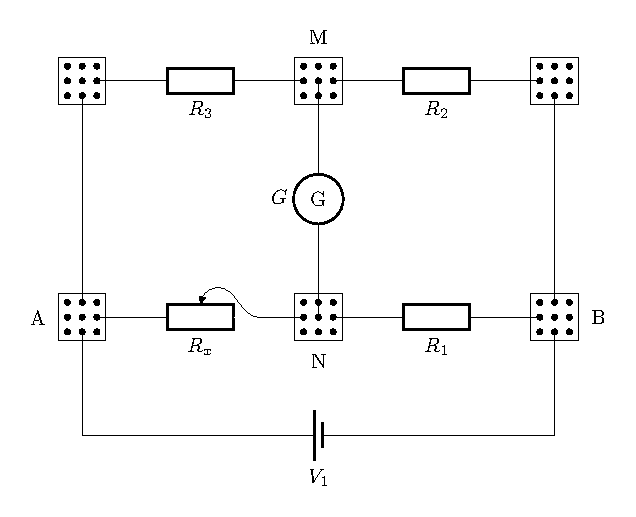
\includegraphics[width=14cm]{fig3.pdf}
\end{figure}

 منبع $V_2$ و مقاومت $R_4$ را با یک گالوانومتر و مقاومت $R_5$ را با یک رئوستا (مقاومت مجهول $R_x$ جایگزین کردیم و  مقاومت رئوستا را تغییر دادیم طوری که گالوانومتر جریان صفر را نشان دهد. در این حالت، اختلاف پتانسیل دو سر مقاومت $R_x$ و جریان عبوری از آن را اندازه‌گیری کرده و در جدول 5 ثبت کردیم.

%\end{wraptable}{l}{4cm} % r = راست جدول، 4cm = پهنای جدول
%\vspace{-10pt} % برای تنظیم فاصله عمودی (اختیاری)
\begin{table}[h!]
\caption{}
\label{tab4}
\centering
\begin{tabular}{cc}
\hline
$V_{R_x} \;[\mathrm{V}]$ & $0.886$ \\
\hline
$I_{R_x} \;[\mathrm{mA}]$ & $10.93$ \\
\hline
\end{tabular}
\end{table}
%\end{wraptable}

با استفاده از جدول $R_x$ را محاسبه می‌کنیم. همچنین با استفاده از رابطه مقاومت‌ها برای پل وتستون مقاومت مجهول را محاسبه می‌کنیم. و بررسی می‌کنیم که آیا اختلافی بین این دو مقدار وجود دارد؟ در نهایت درصد خطای $R_x$ اول را نسبت به $R_x$ دوم محاسبه می‌کنیم.

در حالت تعادل پل (یعنی زمانی که گالوانومتر جریان صفر نشان داد)، اختلاف پتانسیل دو سر مقاومت مجهول و جریان عبوری از آن مطابق جدول \ref{tab4} اندازه‌گیری شد. بنابراین با استفاده از قانون اهم، مقدار مقاومت مجهول از روش مستقیم به‌صورت زیر به‌دست آمد:
\begin{equation}
R_{x,1}=\frac{V_{R_x}}{I_{R_x}}.
\end{equation}
با جایگذاری مقادیر اندازه‌گیری‌شده:
\[
V_{R_x}=0.886~\mathrm{V}, \qquad I_{R_x}=10.93~\mathrm{mA}=10.93\times 10^{-3}~\mathrm{A},
\]
خواهیم داشت:
\begin{align}
R_{x,1}
&=\frac{0.886}{10.93\times 10^{-3}}~\Omega
=\frac{0.886}{0.01093}~\Omega \nonumber\\
&= 81.06~\Omega.
\end{align}

\paragraph{محاسبهٔ \texorpdfstring{$R_x$}{Rx} با رابطهٔ پل وتستون}

در حالت تعادل پل وتستون، جریان گالوانومتر صفر است و در نتیجه پتانسیل دو گرهٔ میانی برابر می‌شود. لذا نسبت مقاومت‌ها در دو شاخهٔ پل مطابق شکل (3) برقرار است. با توجه به آرایش مقاومت‌ها در شکل (2)، رابطهٔ تعادل به صورت زیر نوشته شد:
\begin{equation}
\frac{R_1}{R_2}=\frac{R_x}{R_3}
\qquad \Longrightarrow \qquad
R_{x,2}=\frac{R_1R_3}{R_2}.
\end{equation}
با جایگذاری مقادیر اندازه‌گیری‌شدهٔ مقاومت‌ها از جدول \ref{tab1}:
\[
R_1=388~\Omega,\qquad R_2=219~\Omega,\qquad R_3=47~\Omega,
\]
داریم:
\begin{align}
R_{x,2}
&=\frac{388\times 47}{219}~\Omega
=\frac{18236}{219}~\Omega \nonumber\\
&=83.27~\Omega.
\end{align}

\paragraph{مقایسهٔ دو مقدار و محاسبهٔ درصد خطا}

دو مقدار محاسبه‌شده برای مقاومت مجهول به صورت زیر است:
\[
R_{x,1}=81.06~\Omega, 
\qquad
R_{x,2}=83.27~\Omega.
\]
اختلاف بین این دو مقدار به‌صورت زیر قابل محاسبه است:
\[
\Delta R = |R_{x,1}-R_{x,2}| = |81.06-83.27| = 2.21~\Omega.
\]
درصد خطای روش اول نسبت به روش پل وتستون (به‌عنوان مرجع) از رابطهٔ زیر به‌دست آمد:
\begin{equation}
\%\text{خطا}=
\left|
\frac{R_{x,1}-R_{x,2}}{R_{x,2}}
\right|\times 100,
\end{equation}
بنابراین:
\begin{align}
\%\text{خطا}
&=
\left|
\frac{81.06-83.27}{83.27}
\right|\times 100 \nonumber\\
&=2.65\%.
\end{align}

اختلاف مشاهده‌شده بین دو مقدار \lr{$R_{x,1}$} و \lr{$R_{x,2}$} می‌تواند ناشی از خطای اندازه‌گیری ولتاژ و جریان (دقت محدود ولت‌متر و آمپرمتر)، مقاومت داخلی گالوانومتر و سیم‌های رابط، تلرانس مقاومت‌های \lr{$R_1,R_2,R_3$}، و همچنین عدم رسیدن دقیق به حالت تعادل (صفرِ کامل گالوانومتر) باشد. با این حال، با توجه به مقدار خطای به‌دست‌آمده (حدود چند درصد)، می‌توان نتیجه گرفت که دو روش با یکدیگر سازگاری مناسبی دارند و پل وتستون روش دقیق‌تری برای اندازه‌گیری مقاومت مجهول فراهم می‌کند.
 


\section*{پرسش‌ها}
\paragraph{1} رابطه $R_1 R_3 = R_x R_2$ را در مدار شکل 2 اثبات کنید


در مدار پل وتستونِ شکل (۳)، در حالت تعادل گالوانومتر جریان صفر نشان می‌دهد؛ بنابراین جریان عبوری از شاخهٔ میانی (گالوانومتر) صفر است:
\begin{equation}
I_g = 0.
\end{equation}
صفر بودن جریان گالوانومتر به این معناست که دو گرهٔ متصل به دو سر گالوانومتر هم‌پتانسیل‌اند. اگر این دو گره را به‌ترتیب $B$ و $D$ بنامیم، خواهیم داشت:
\begin{equation}
V_B = V_D.
\label{eq:VBVD}
\end{equation}

اکنون فرض می‌شود منبع تغذیه بین دو سر پل (مثلاً گره‌های $A$ و $C$) قرار دارد و دو شاخهٔ کناری شامل مقاومت‌های
\[
A \to B \to C \quad : \quad R_1 \ \text{و}\ R_2,
\qquad
A \to D \to C \quad : \quad R_3 \ \text{و}\ R_x
\]
هستند (مطابق نام‌گذاری شکل ۳). در این حالت، چون از گالوانومتر جریانی عبور نمی‌کند، دو شاخهٔ چپ و راست از نظر جریان مستقل‌اند؛ بنابراین جریان عبوری از $R_1$ و $R_2$ را برابر $I_L$ و جریان عبوری از $R_3$ و $R_x$ را برابر $I_R$ می‌گیریم:
\begin{equation}
I_{R_1}=I_{R_2}=I_L,
\qquad
I_{R_3}=I_{R_x}=I_R.
\end{equation}

از قانون اهم برای افت ولتاژ روی مقاومت‌ها استفاده می‌کنیم. با توجه به \eqref{eq:VBVD} داریم:
\begin{align}
V_A - V_B &= I_L R_1,
&
V_A - V_D &= I_R R_3,
\\
V_B - V_C &= I_L R_2,
&
V_D - V_C &= I_R R_x.
\end{align}
از برابر بودن پتانسیل‌های $B$ و $D$ نتیجه می‌شود:
\begin{equation}
V_A - V_B = V_A - V_D
\quad \Longrightarrow \quad
I_L R_1 = I_R R_3,
\label{eq:1}
\end{equation}
و نیز:
\begin{equation}
V_B - V_C = V_D - V_C
\quad \Longrightarrow \quad
I_L R_2 = I_R R_x.
\label{eq:2}
\end{equation}

اکنون با تقسیم رابطهٔ \eqref{eq:1} بر \eqref{eq:2} داریم:
\begin{equation}
\frac{I_L R_1}{I_L R_2} = \frac{I_R R_3}{I_R R_x}
\quad \Longrightarrow \quad
\frac{R_1}{R_2} = \frac{R_3}{R_x}.
\end{equation}
با ضرب طرفین در $R_2 R_x$ نتیجه می‌شود:
\begin{equation}
R_1 R_x = R_2 R_3.
\label{eq:balance}
\end{equation}

حال اگر در شکل (۳) جای‌گذاری مقاومت مجهول و مقاومت $R_3$ به‌گونه‌ای باشد که نسبت‌ها به صورت
\[
\frac{R_1}{R_2}=\frac{R_x}{R_3}
\]
تعریف شده باشد (که صرفاً به نحوهٔ نام‌گذاری گره‌ها و چیدمان مقاومت‌ها در شکل بستگی دارد)، آنگاه به‌سادگی از همان روند بالا رابطهٔ زیر به‌دست می‌آید:
\begin{equation}
R_1 R_3 = R_x R_2.
\end{equation}
بنابراین، رابطهٔ تعادل پل وتستون نتیجهٔ مستقیم هم‌پتانسیل شدن دو گرهٔ میانی در حالت جریان صفر گالوانومتر و به‌کارگیری قانون اهم در دو شاخهٔ پل است.


\end{document}